
\clearpage
\section*{Solutions}
\small
\subsection*{1(a). Verifying a dominating set}
Let $n=|V|$ and $m=|E|$. I first check that $D$ has at most $k$ vertices and contains only vertices in the graph. I then collect the selected vertices and all their neighbors. If this covers all of $V$, I return true. This also handles disconnected graphs: an isolated vertex must be selected because it has no neighbor that could cover it.
\begin{lstlisting}[language=Python]
def checkDominatingSet(G, D, k):
  #you may, but are not required to, convert G to a networkx graph
  H = nx.Graph()
  H.add_edges_from(G[1])
  H.add_nodes_from(G[0])

  chosen = set(D)
  if len(chosen) > k or not chosen <= set(H.nodes()):
    return False
  covered = set(chosen)
  for u in chosen:
    covered.update(H.neighbors(u))
  return len(covered) == len(H)
\end{lstlisting}

If the function returns true, each vertex is selected or adjacent to a selected vertex, and the size bound holds. Conversely, a dominating set of size at most $k$ passes the size and membership checks and covers every vertex, so the function returns true. With hash sets and adjacency lists, the expected runtime is $O(n+m+|D|)$, or $O(n+m)$ when $D\subseteq V$; auxiliary space is $O(n+m)$ including the NetworkX graph. The neighbor scans total at most $2m$.

\subsection*{1(b). NP-completeness via Vertex Cover}
Dominating Set is in NP because I can verify a proposed set in polynomial time using part (a). To show NP-hardness, I reduce Vertex Cover to Dominating Set. For a simple undirected graph, I remove isolated vertices, since they do not affect a vertex cover. I keep every original edge $uv$ and add a new vertex $w_{uv}$ connected to both endpoints. Each original edge is now part of a triangle.
\begin{lstlisting}
VertexCoverUsingDominatingSet(G, k):
    if k < 0: return False
    U = vertices of G with positive degree
    H = graph with vertices U and all original edges
    for each edge {u,v} in G:
        create a fresh vertex w_uv in H
        add edges {u,w_uv} and {v,w_uv} to H
    D = findDominatingSet(H)
    return (|D| <= k)
\end{lstlisting}
If $C$ is a vertex cover of $G$, it dominates every $w_{uv}$ because it contains $u$ or $v$. It also dominates every original nonisolated vertex: a vertex outside $C$ has a neighbor in $C$ along any incident edge. Thus $C$ dominates $H$.

Conversely, take any dominating set $D$ of $H$. Replace each chosen $w_{uv}$ with $u$, discarding duplicates. This does not increase its size or lose domination: $N_H[w_{uv}]=\{w_{uv},u,v\}\subseteq N_H[u]$, since $uv$ was retained. The resulting set $C$ consists only of original vertices. Each $w_{uv}$ must now have $u$ or $v$ in $C$, so $C$ covers every original edge. Hence $G$ has a cover of size at most $k$ if and only if $H$ has a dominating set of size at most $k$. An edgeless input produces an empty $H$, correctly accepting exactly when $k\geq0$.

The constructed graph has at most $n+m$ vertices and exactly $3m$ edges. Construction and comparison take $O(n+m)$ time and space, with one oracle call. If its time is $T_{\rm DS}(N,M)$, total time is $O(n+m)+T_{\rm DS}(n'+m,3m)$, where $n'\leq n$ counts nonisolated vertices. Thus a polynomial-time minimum-dominating-set algorithm would yield a polynomial-time Vertex Cover algorithm. Together with NP membership, this establishes NP-completeness of the decision problem.

\clearpage
\subsection*{2(a). Greedy dominating set}
My greedy algorithm selects the vertex that covers the most currently undominated vertices, counting the vertex itself. I mark those vertices covered and repeat until none remain. On a tie, I take the first vertex in NetworkX insertion order. Since the graph setup adds edges before the node list, the edge order affects this tie rule.
\begin{lstlisting}[language=Python]
def greedyDominatingSet(G):
  #you may, but are not required to, convert G to a networkx graph
  H = nx.Graph()
  H.add_edges_from(G[1])
  H.add_nodes_from(G[0])

  uncovered = set(H.nodes())
  closed = {v: set(H.neighbors(v)) | {v} for v in H}
  result = []
  while uncovered:
    # max keeps the first vertex in insertion order on a tie.
    v = max(H.nodes(), key=lambda u: len(closed[u] & uncovered))
    result.append(v)
    uncovered.difference_update(closed[v])
  return result
\end{lstlisting}

While any vertex remains uncovered, some candidate covers at least itself, so each iteration makes progress. The process stops in at most $n$ iterations and returns a dominating set. Each iteration evaluates all closed neighborhoods; their total size is $n+2m$, so the expected runtime is $O(n(n+m))$ with hash sets. Space is $O(n+m)$.

\subsection*{2(b). Greedy counterexample}
For my example, I use $V=[0,1,2,3,4,5]$ and add the edges in this order:
\[
 E=[(0,4),(0,5),(1,2),(1,3),(1,4),(2,3),(2,4)].
\]
\begin{center}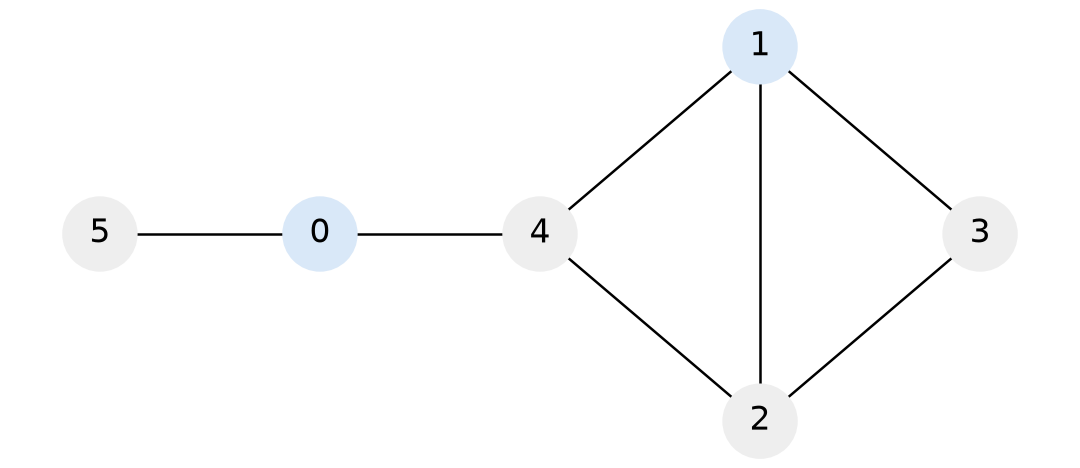
\includegraphics[width=.72\linewidth]{greedy_counterexample.png}\end{center}
The setup inserts vertices in order $[0,4,5,1,2,3]$. Initially vertices $4,1,2$ each cover four vertices, so the tie rule selects $4$. Its closed neighborhood is $\{0,1,2,4\}$, leaving $\{3,5\}$ uncovered. Every candidate that covers an uncovered vertex now gains one; vertex $0$ is first in insertion order, so it is selected and covers $5$. Finally $1$ is the first candidate covering the remaining vertex $3$. The returned sequence is $[4,0,1]$.

But $\{0,1\}$ dominates the graph: $N[0]=\{0,4,5\}$ and $N[1]=\{1,2,3,4\}$. No vertex has degree five, so no single vertex dominates all six vertices; the minimum size is two. I can also remove $4$ from the greedy output and still have a dominating set. So the result is neither minimum in size nor minimal under removing vertices.

\clearpage
\subsection*{3(a). Individuals}
I represent each individual as a binary list of length $n$. A one at position $i$ means I selected the $i$th vertex in NetworkX node order; a zero means I left it out. I generate each initial bit independently with equal probability of zero or one. Keeping a fixed node order lets me use the same representation even when vertex labels are not consecutive integers.
\begin{lstlisting}[language=Python]
def randomIndividual(G):
  # Position i represents the ith vertex in G.nodes() order.
  n = len(G.nodes()) if isinstance(G, nx.Graph) else len(G[0])
  return np.random.randint(0, 2, size=n).tolist()
\end{lstlisting}

\subsection*{3(b). Selection, recombination, and mutation}
I use roulette-wheel selection, so each parent's probability of being selected is proportional to its fitness. I select with replacement, meaning the same individual can be chosen twice. For recombination, I choose an interior cut at random and swap the parents' suffixes to produce two children. I copy individuals with fewer than two genes. Each child bit mutates independently with probability $1/n$, and I use $1/\max(1,n)$ to handle an empty graph. I also keep the best individual unchanged in each generation.
\begin{lstlisting}[language=Python]
def selection(pop, fitnesses):
  weights = np.asarray(fitnesses, dtype=float)
  if len(pop) == 0 or len(weights) != len(pop):
    raise ValueError("Population and fitnesses must be nonempty and aligned")
  if not np.all(np.isfinite(weights)) or np.any(weights < 0):
    raise ValueError("Fitness weights must be finite and nonnegative")
  total = weights.sum()
  probabilities = weights / total if total > 0 else None
  i, j = np.random.choice(len(pop), size=2, replace=True, p=probabilities)
  return list(pop[i]), list(pop[j])
\end{lstlisting}
\begin{lstlisting}[language=Python]
def recombine(a, b):
  if len(a) != len(b):
    raise ValueError("Parents must have equal lengths")
  if len(a) < 2:
    return list(a), list(b)
  cut = np.random.randint(1, len(a))
  return list(a[:cut]) + list(b[cut:]), list(b[:cut]) + list(a[cut:])
\end{lstlisting}
\begin{lstlisting}[language=Python]
def mutate(ind, p=0.1):
  if not 0 <= p <= 1:
    raise ValueError("Mutation probability must be between 0 and 1")
  for i in range(len(ind)):
    if np.random.random() < p:
      ind[i] = 1 - ind[i]
  return ind
\end{lstlisting}

\clearpage
\subsection*{3(c). Fitness}
I use $s$ for the number of selected vertices and $u$ for the number of undominated vertices. My fitness function is
\[
 f=\frac{1}{1+s+(n+1)u}.
\]
I maximize this value. It is always positive, so I can use it directly for roulette-wheel selection. Every feasible individual has fitness at least $1/(n+1)$, whereas any infeasible individual has fitness at most $1/(n+2)$. Thus every dominating set outranks every infeasible individual. Among dominating sets, fewer selected vertices gives strictly higher fitness. Evaluation takes $O(n+m)$ expected time.
\begin{lstlisting}[language=Python]
def evalFitness(ind, G):
  H = G if isinstance(G, nx.Graph) else nx.Graph()
  if not isinstance(G, nx.Graph):
    H.add_nodes_from(G[0])
    H.add_edges_from(G[1])
  nodes = list(H.nodes())
  if len(ind) != len(nodes) or any(bit not in (0, 1) for bit in ind):
    raise ValueError("Individual must have one binary gene per vertex")
  chosen = {v for v, bit in zip(nodes, ind) if bit}
  covered = set(chosen)
  for v in chosen:
    covered.update(H.neighbors(v))
  missing = len(nodes) - len(covered)
  return 1.0 / (1 + len(chosen) + (len(nodes) + 1) * missing)
\end{lstlisting}

\subsection*{Generation update}
I record the population's minimum, average, and maximum fitness before creating the next generation. The plot therefore shows generations $0$ through $999$. After the last update, I evaluate the final population and return its best individual.
\begin{lstlisting}[language=Python]
def runGA(G, popSize=10, generations=100):
  #you may, but are not required to, convert G to a networkx graph
  H = nx.Graph()
  H.add_edges_from(G[1])
  H.add_nodes_from(G[0])

  if popSize < 1 or generations < 0:
    raise ValueError("Population must be positive and generations nonnegative")
  pop = [randomIndividual(H) for _ in range(popSize)]
  fitnessList = [] #each element is (min, avg, max) fitness for a generation

  for gen in range(generations):
    print('Generation', gen)
    fitnesses = [evalFitness(ind, H) for ind in pop]
    fitnessList.append((min(fitnesses), np.mean(fitnesses), max(fitnesses)))
    newPop = []
    # Preserve the best individual and create the remaining population.
    elite = max(range(len(pop)), key=lambda i: fitnesses[i])
    newPop.append(list(pop[elite]))
    while len(newPop) < popSize:
      a, b = selection(pop, fitnesses)
      for child in recombine(a, b):
        mutate(child, p=1.0 / max(1, len(H)))
        newPop.append(child)
        if len(newPop) == popSize:
          break
    pop = newPop

  bestSol, bestFitness = max([(ind, evalFitness(ind, H)) for ind in pop], key=lambda x: x[1])
  return bestSol, bestFitness, fitnessList
\end{lstlisting}

\clearpage
\subsection*{3(d). Results and observations}
I ran the algorithm on \texttt{nx.path\_graph(100)}, matching the skeleton's 100-vertex path. I used a population of 50 for 1000 generations and set NumPy's random seed to 650 so I could reproduce the run.
\begin{center}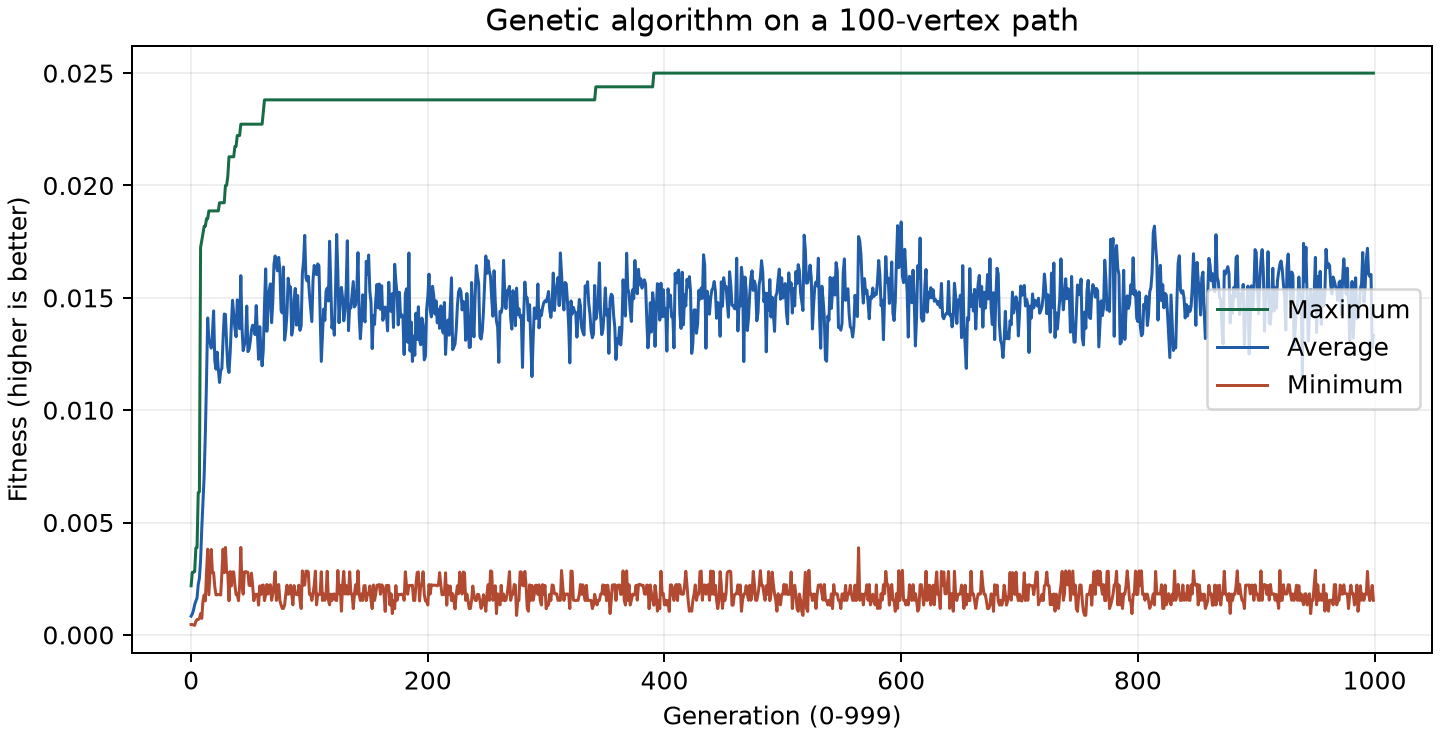
\includegraphics[width=.94\linewidth]{fitness.png}\end{center}
The recorded summary statistics are approximately
\begin{center}
\begin{tabular}{r|rrr}
Generation & Minimum & Average & Maximum\\\hline
0 & 0.000460 & 0.000834 & 0.002183\\
999 & 0.001541 & 0.013331 & 0.025000
\end{tabular}
\end{center}
My final solution is a valid dominating set with 39 vertices and fitness $1/40=0.025$. The selected vertices are
\begin{quote}\small
1, 2, 5, 8, 11, 14, 17, 20, 23, 25, 28, 31, 34, 36, 38, 41, 42, 45, 48, 51, 53, 56, 59, 62, 64, 66, 68, 70, 72, 75, 76, 79, 82, 84, 87, 89, 92, 95, 98.
\end{quote}
In my run, the maximum fitness rises in steps and never decreases because I preserve the best individual. The average improves overall, but it still fluctuates. The minimum stays low because crossover and mutation can leave vertices uncovered, which causes a large fitness penalty. Once the population finds valid dominating sets, their higher fitness makes them more likely to reproduce. The later plateaus show that improvements become less frequent.

My run did not reach the optimum. Each chosen vertex on a path covers at most three vertices, so at least $\lceil100/3\rceil=34$ vertices are necessary. The set $\{1,4,7,\ldots,97,99\}$ has 34 vertices and dominates the path, proving that bound is achievable. My solution uses five more vertices than the optimum. The run finds a small dominating set, but the genetic algorithm does not guarantee the smallest one.
